% =====================================================================
% IBFE Tutorials: solid mechanics preparation
% =====================================================================
\documentclass[aspectratio=169,11pt]{beamer}

% Match the visual language of the SIAM Waves talk.
\usetheme{Boadilla}
\usecolortheme{seahorse}
\useinnertheme{rectangles}
\useoutertheme{infolines}

\setbeamercolor{structure}{fg=blue!55!black}
\setbeamercolor{title}{fg=white,bg=blue!55!black}
\setbeamercolor{frametitle}{fg=blue!55!black}
\setbeamercolor{block title}{bg=blue!12,fg=blue!55!black}
\setbeamercolor{block body}{bg=blue!4}
\setbeamertemplate{navigation symbols}{}
\setbeamerfont{frametitle}{series=\bfseries,size=\large}
\setbeamerfont{title}{series=\bfseries,size=\Large}

\usepackage[T1]{fontenc}
\usepackage[utf8]{inputenc}
\DeclareFontShape{T1}{cmss}{b}{n}{<->ssub*cmss/bx/n}{}
\usepackage{graphicx}
% These prefixes allow compilation from either the repository root or this folder.
\graphicspath{{./}{../}}
\usepackage{amsmath,amssymb,bm,mathtools}
\usepackage{booktabs}
\usepackage{xcolor}
\usepackage{tikz}
\usetikzlibrary{arrows.meta,calc}
\usepackage{tcolorbox}
\tcbuselibrary{skins}
\usepackage{hyperref}
\hypersetup{colorlinks=true,urlcolor=blue!55!black}

\newcommand{\hi}[1]{\textcolor{blue!55!black}{\textbf{#1}}}
\newcommand{\warn}[1]{\textcolor{red!70!black}{\textbf{#1}}}
\newcommand{\soft}[1]{\textcolor{gray!50!black}{#1}}
\newcommand{\R}{\mathbb{R}}
\newcommand{\X}{\bm{X}}
\newcommand{\x}{\bm{x}}
\newcommand{\I}{\bm{I}}
\newcommand{\uEuler}{\bm{u}}
\newcommand{\Fdef}{\bm{F}_{\chi}}
\newcommand{\Cten}{\bm{C}}
\newcommand{\Bten}{\bm{B}}
\newcommand{\Eten}{\bm{E}}
\newcommand{\eten}{\bm{e}}
\newcommand{\sigmaC}{\bm{\sigma}}
\newcommand{\Pten}{\bm{P}}
\newcommand{\Sten}{\bm{S}}
\newcommand{\Nvec}{\bm{N}}
\newcommand{\nvec}{\bm{n}}
\newcommand{\tvec}{\bm{t}}
\newcommand{\FLag}{\bm{F}}
\newcommand{\fEuler}{\bm{f}}
\newcommand{\gradX}{\nabla_{\!X}}
\newcommand{\gradx}{\nabla_{\!x}}
\newcommand{\divx}{\nabla_{\!x}\!\cdot}

\newtcolorbox{punchbox}{
  enhanced,
  colback=blue!4,
  colframe=blue!55!black,
  boxrule=0.6pt,
  arc=2pt,
  left=4pt,right=4pt,top=3pt,bottom=3pt
}

\title[Solid mechanics for IBFE]{Solid mechanics for IBFE}
\subtitle{Kinematics, strain, stress, and hyperelasticity}
\author[Miller]{Laura A. Miller}
\institute[UArizona]{Department of Mathematics, University of Arizona}
\date{}

\begin{document}

% ----- 1. Title -----
\begin{frame}[plain]
  \begin{beamercolorbox}[sep=10pt,center]{title}
    {\bfseries\Large Solid mechanics for IBFE}\\[3pt]
    {\normalsize Kinematics, strain, stress, and hyperelasticity}
  \end{beamercolorbox}
  \vspace{1.35em}
  \begin{columns}[T,onlytextwidth]
  \begin{column}{0.55\textwidth}
    \textbf{\large Laura A. Miller}\\[4pt]
    Department of Mathematics\\
    University of Arizona\\[14pt]
    {\small IBFE Tutorials}
  \end{column}
  \begin{column}{0.45\textwidth}
    \begin{punchbox}
      \centering
      \[
        \chi
        \;\longrightarrow\;
        \Fdef
        \;\longrightarrow\;
        W
        \;\longrightarrow\;
        \Pten
      \]
      \small motion, deformation, energy, stress
    \end{punchbox}
  \end{column}
  \end{columns}
  \vfill
  \centering{\tiny\color{black!55}AI tools were used to assist with formatting, organization, and clarification of the instructor's original notes.}
\end{frame}

% ----- 3. Overview -----
\begin{frame}{Roadmap}
\begin{columns}[T,onlytextwidth]
\begin{column}{0.49\textwidth}
\begin{enumerate}\itemsep6pt
  \item Notation and tensor bookkeeping
  \item Configurations and the deformation map
  \item Finite strain measures
  \item Stress measures and transformations
\end{enumerate}
\end{column}
\begin{column}{0.49\textwidth}
\begin{enumerate}\setcounter{enumi}{4}\itemsep6pt
  \item Hyperelasticity and the IBFE force pipeline
  \item Worked axial-deformation example
  \item Neo-Hookean stress derivation and checks
\end{enumerate}
\end{column}
\end{columns}
\begin{punchbox}
\centering
\[
  \chi\longrightarrow\Fdef,J
  \longrightarrow\Cten,\Eten
  \longrightarrow W
  \longrightarrow\Pten
  \longrightarrow\FLag
  \longrightarrow\fEuler .
\]
\end{punchbox}
\end{frame}

\section{Notation and tensor bookkeeping}

% ----- 4. Module 0 -----
\begin{frame}{Module 0: purpose and scope}
\begin{columns}[T,onlytextwidth]
\begin{column}{0.57\textwidth}
\textbf{Goal}

Build the minimum solid-mechanics toolkit needed to follow IBFE derivations.

\medskip
\textbf{Audience}

Advanced undergraduates and graduate students who are new to continuum mechanics.
\end{column}
\begin{column}{0.43\textwidth}
\begin{punchbox}
\small
This module establishes:
\begin{itemize}\itemsep4pt
  \item reference and current coordinates,
  \item tensor types and indices,
  \item material and spatial derivatives,
  \item distinct symbols for deformation and force.
\end{itemize}
\end{punchbox}
\end{column}
\end{columns}
\end{frame}

% ----- 5. Coordinates -----
\begin{frame}{Configurations, coordinates, and fields}
\begin{columns}[T,onlytextwidth]
\begin{column}{0.54\textwidth}
\begin{itemize}\itemsep6pt
  \item \hi{Reference configuration}: \(B_0\subset\R^d\), with material coordinate \(\X\).
  \item \hi{Current configuration}: \(B_t\subset\R^d\), with spatial coordinate \(\x\).
  \item \hi{Motion}: \(\chi(\cdot,t):B_0\to B_t\), with
  \[
    \x=\chi(\X,t).
  \]
\end{itemize}
\begin{punchbox}
\small
Material fields use \(\X\) as their independent coordinate. Spatial fields use \(\x\).
\end{punchbox}
\end{column}
\begin{column}{0.46\textwidth}
\centering
\includegraphics[width=\linewidth]{pictures/4-2/ref-current.png}\\
\soft{\scriptsize A material point keeps its label \(\X\) while its current position changes.}
\end{column}
\end{columns}
\end{frame}

% ----- 6. Tensor primer -----
\begin{frame}{Scalars, vectors, and second-order tensors}
\begin{center}
\renewcommand{\arraystretch}{1.28}
\begin{tabular}{lll}
\toprule
Object & Components & Example \\
\midrule
Scalar & \(a\) & energy density \(W\) \\
Vector & \(v_i\) or \(v_I\) & velocity, normal, force \\
Spatial tensor & \(A_{ij}\) & Cauchy stress \(\sigma_{ij}\) \\
Material tensor & \(A_{IJ}\) & Green strain \(E_{IJ}\) \\
Two-point tensor & \(A_{iI}\) & \((F_\chi)_{iI}\), \(P_{iI}\) \\
\bottomrule
\end{tabular}
\end{center}
\begin{punchbox}
\small
A two-point tensor maps a material direction into a spatial direction. Both the deformation gradient and first Piola stress have one spatial and one material index.
\[
  i,j,k:\ \text{spatial},
  \qquad
  I,J,K:\ \text{material}.
\]
Repeated indices are summed unless stated otherwise.
\end{punchbox}
\end{frame}

% ----- 7. Field table -----
\begin{frame}{Material and spatial fields}
\small
\begin{center}
\renewcommand{\arraystretch}{1.2}
\begin{tabular}{ll}
\toprule
Reference domain \(B_0\) & Current domain \(B_t\) or fluid domain \(\Omega\) \\
\midrule
\(\X\): material coordinate & \(\x\): spatial coordinate \\
\(\chi(\X,t)\): motion & \(\uEuler(\x,t)\): velocity \\
\(\Fdef=\gradX\chi\): deformation gradient & \(\sigmaC(\x,t)\): Cauchy stress \\
\(J=\det\Fdef\): volume ratio & \(p(\x,t)\): pressure \\
\(\Pten(\X,t)\): first Piola stress & \(\fEuler(\x,t)\): Eulerian force density \\
\(\FLag(\X,t)\): Lagrangian force density & \\
\bottomrule
\end{tabular}
\end{center}
\begin{punchbox}
\small
Always check the independent coordinate before differentiating or integrating a field.
\end{punchbox}
\end{frame}

% ----- 9. Derivatives -----
\begin{frame}{Material and spatial derivatives}
\begin{columns}[T,onlytextwidth]
\begin{column}{0.50\textwidth}
\begin{block}{Material gradient}
\[
  \gradX(\cdot)
\]
differentiates with respect to \(\X\). For the motion,
\[
  (\gradX\chi)_{iI}
  =\frac{\partial\chi_i}{\partial X_I}.
\]
\end{block}
\end{column}
\begin{column}{0.48\textwidth}
\begin{block}{Spatial gradient}
\[
  \gradx(\cdot)
\]
differentiates with respect to \(\x\). For velocity,
\[
  (\gradx\uEuler)_{ij}
  =\frac{\partial u_i}{\partial x_j}.
\]
\end{block}
\end{column}
\end{columns}
\begin{punchbox}
\small
IBFE structural kinematics and constitutive stress are normally evaluated on \(B_0\), so \(\gradX\) appears throughout the finite-element formulation.
\end{punchbox}
\end{frame}

% ----- 10. Symbol distinction -----
\begin{frame}{Deformation gradient and Lagrangian force}
IB and IBFE papers often use bold \(F\) for a Lagrangian force density, while solid-mechanics texts use bold \(F\) for the deformation gradient.
\begin{columns}[T,onlytextwidth]
\begin{column}{0.49\textwidth}
\begin{block}{Kinematics}
\[
  \Fdef(\X,t):=\gradX\chi(\X,t)
\]
is a two-point tensor.
\end{block}
\end{column}
\begin{column}{0.49\textwidth}
\begin{block}{Forcing}
\[
  \FLag(\X,t)
\]
is a Lagrangian vector force density.
\end{block}
\end{column}
\end{columns}
\begin{punchbox}
\centering
\[
  \Fdef\neq\FLag .
\]
\small The subscript on \(\Fdef\) keeps kinematics distinct from forcing.
\end{punchbox}
\end{frame}

\section{Configurations and the deformation map}

% ----- 10. Module 1 -----
\begin{frame}{Module 1: configurations and motion}
\begin{columns}[T,onlytextwidth]
\begin{column}{0.52\textwidth}
\[
  \chi(\cdot,t):B_0\to B_t,
  \qquad
  \x=\chi(\X,t).
\]
The displacement is
\[
  \bm{d}(\X,t)=\chi(\X,t)-\X.
\]
\end{column}
\begin{column}{0.46\textwidth}
\begin{punchbox}
\small
This module develops two local measures from the motion:
\[
  \Fdef=\gradX\chi,
  \qquad
  J=\det\Fdef.
\]
\(\Fdef\) maps line elements and \(J\) maps volume elements.
\end{punchbox}
\end{column}
\end{columns}
\end{frame}

% ----- 11. Nearby points -----
\begin{frame}{Nearby material points under the motion}
\begin{columns}[T,onlytextwidth]
\begin{column}{0.48\textwidth}
Choose neighboring material points
\[
  \X,\qquad \X+d\X .
\]
Their current positions are
\[
  \x=\chi(\X,t),
  \qquad
  \x+d\x=\chi(\X+d\X,t).
\]
Thus
\[
  d\x
  =
  \chi(\X+d\X,t)-\chi(\X,t).
\]
\begin{punchbox}
\small
The deformation gradient is the linear map that approximates this change for small \(d\X\).
\end{punchbox}
\end{column}
\begin{column}{0.52\textwidth}
\centering
\includegraphics[width=\linewidth]{pictures/4-2/def-tensor.png}
\end{column}
\end{columns}
\end{frame}

% ----- 12. F definition -----
\begin{frame}{Deformation-gradient definition}
Linearizing the motion about \(\X\) gives
\[
  d\x=\Fdef(\X,t)\,d\X+o(\lVert d\X\rVert),
\]
with
\[
  \boxed{\Fdef(\X,t)=\gradX\chi(\X,t)}.
\]
In components,
\[
  (F_\chi)_{iI}
  =\frac{\partial\chi_i}{\partial X_I}.
\]
\begin{columns}[T,onlytextwidth]
\begin{column}{0.48\textwidth}
\textbf{Columns of \(\Fdef\)}

Images of the reference basis vectors.
\end{column}
\begin{column}{0.50\textwidth}
\textbf{Information in \(\Fdef\)}

Stretch, shear, and rotation near one material point.
\end{column}
\end{columns}
\end{frame}

% ----- 13. Inverse -----
\begin{frame}{Inverse differential map at matching points}
\begin{columns}[T,onlytextwidth]
\begin{column}{0.52\textwidth}
\centering
\includegraphics[width=\linewidth]{pictures/4-2/def-tensor.png}
\end{column}
\begin{column}{0.48\textwidth}
If \(\chi(\cdot,t)\) is locally invertible and
\(\x=\chi(\X,t)\), then
\[
  d\X
  =
  \Fdef(\X,t)^{-1}d\x
  +o(\lVert d\x\rVert).
\]
The spatial gradient of the inverse motion is
\[
  \boxed{
  \gradx\chi^{-1}(\x,t)
  =
  \Fdef(\chi^{-1}(\x,t),t)^{-1}
  }.
\]
\begin{punchbox}
\small
The composition with \(\chi^{-1}\) ensures that both tensors refer to the same material point.
\end{punchbox}
\end{column}
\end{columns}
\end{frame}

% ----- 14. J definition -----
\begin{frame}{Jacobian and local volume change}
\[
  \boxed{J(\X,t)=\det\Fdef(\X,t)},
  \qquad
  dv=J\,dV.
\]
\begin{columns}[T,onlytextwidth]
\begin{column}{0.48\textwidth}
\begin{itemize}\itemsep6pt
  \item \(J>1\): local expansion
  \item \(0<J<1\): local compression
  \item \(J=1\): local volume preservation
\end{itemize}
\end{column}
\begin{column}{0.50\textwidth}
\begin{punchbox}
\small
An admissible deformation normally requires
\[
  J>0.
\]
\(J=0\) collapses material volume. \(J<0\) reverses orientation and indicates element inversion.
\end{punchbox}
\end{column}
\end{columns}
\end{frame}

% Figure: local measure change under the motion.
\begin{frame}{Visualizing the Jacobian as a local measure ratio}
\centering
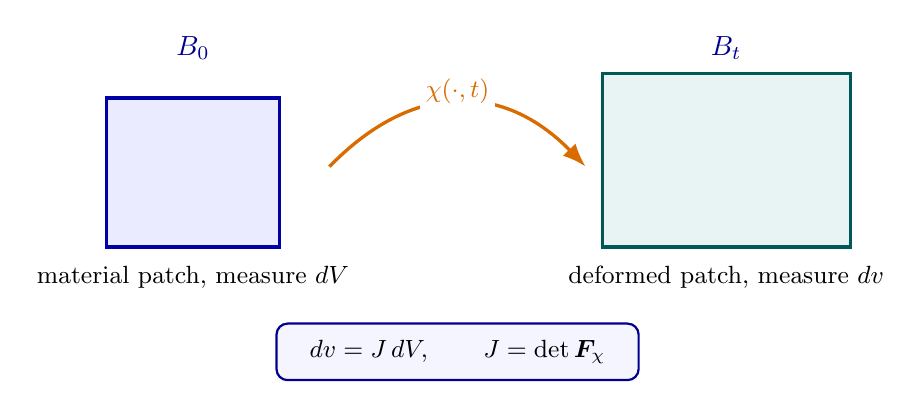
\begin{tikzpicture}[x=1.05cm,y=1.05cm,>=Latex,every node/.style={font=\small}]
  \node[blue!55!black,font=\bfseries] at (-3.2,2.15) {$B_0$};
  \fill[blue!8] (-4.25,-0.25) rectangle (-2.15,1.55);
  \draw[blue!65!black,very thick] (-4.25,-0.25) rectangle (-2.15,1.55);
  \node at (-3.2,-0.62) {material patch, measure $dV$};

  \draw[-{Latex[length=3mm]},very thick,orange!85!black]
    (-1.55,0.72) .. controls (-0.55,1.75) and (0.55,1.75) .. (1.55,0.72);
  \node[orange!85!black,fill=white,inner sep=2pt] at (0,1.63) {$\chi(\cdot,t)$};

  \node[blue!55!black,font=\bfseries] at (3.25,2.15) {$B_t$};
  \fill[teal!9] (1.75,-0.25) rectangle (4.75,1.85);
  \draw[teal!70!black,very thick] (1.75,-0.25) rectangle (4.75,1.85);
  \node at (3.25,-0.62) {deformed patch, measure $dv$};

  \node[draw=blue!55!black,rounded corners,fill=blue!4,thick,
        inner xsep=12pt,inner ysep=6pt] at (0,-1.52)
        {$\displaystyle dv=J\,dV,\qquad J=\det\Fdef$};
\end{tikzpicture}

\vspace{0.25em}
\soft{In two dimensions the corresponding area relation is $da=J\,dA$.}
\end{frame}

% ----- 15. J stretch -----
\begin{frame}{Jacobian as the product of principal stretches}
For a diagonal deformation in \(d\) dimensions,
\[
  \Fdef=\operatorname{diag}(\lambda_1,\ldots,\lambda_d),
  \qquad
  J=\prod_{k=1}^{d}\lambda_k .
\]
\begin{columns}[T,onlytextwidth]
\begin{column}{0.48\textwidth}
\begin{block}{Two dimensions}
\[
  da=J\,dA
  =\lambda_1\lambda_2\,dA .
\]
\end{block}
\end{column}
\begin{column}{0.48\textwidth}
\begin{block}{Three dimensions}
\[
  dv=J\,dV
  =\lambda_1\lambda_2\lambda_3\,dV .
\]
\end{block}
\end{column}
\end{columns}
\begin{punchbox}
\small
Volume preservation does not imply zero strain. A simple shear has \(J=1\) and still changes angles and lengths.
\end{punchbox}
\end{frame}

% ----- 16. Micro-check prompt -----
\begin{frame}{Micro-check: deformation gradients and Jacobians}
\begin{columns}[T,onlytextwidth]
\begin{column}{0.49\textwidth}
\begin{block}{A. Uniform stretch}
\[
  \chi(\X)
  =
  (\lambda X_1,\lambda X_2,\lambda X_3).
\]
\begin{enumerate}\itemsep5pt
  \item Compute \(\Fdef=\gradX\chi\).
  \item Compute \(J=\det\Fdef\).
  \item Interpret the volume change.
\end{enumerate}
\end{block}
\end{column}
\begin{column}{0.49\textwidth}
\begin{block}{B. Simple shear}
\[
  \chi(\X)
  =
  (X_1+\gamma X_2,X_2,X_3).
\]
\begin{enumerate}\itemsep5pt
  \item Compute each \((F_\chi)_{iI}\).
  \item Compute \(J\).
  \item Decide whether the map is strain free.
\end{enumerate}
\end{block}
\end{column}
\end{columns}
\end{frame}

% ----- 17. Uniform stretch solution -----
\begin{frame}{Micro-check solution: uniform stretch}
From
\[
  \chi_1=\lambda X_1,\qquad
  \chi_2=\lambda X_2,\qquad
  \chi_3=\lambda X_3,
\]
we obtain
\[
  \Fdef
  =
  \begin{bmatrix}
    \lambda&0&0\\
    0&\lambda&0\\
    0&0&\lambda
  \end{bmatrix}
  =\lambda\I .
\]
Therefore
\[
  \boxed{J=\det\Fdef=\lambda^3}.
\]
\begin{punchbox}
\small
Every length scales by \(\lambda\), every area by \(\lambda^2\), and every volume by \(\lambda^3\).
\end{punchbox}
\end{frame}

% ----- 18. Shear solution -----
\begin{frame}{Micro-check solution: simple shear}
For
\[
  \chi(\X)
  =
  (X_1+\gamma X_2,X_2,X_3),
\]
\[
  \Fdef
  =
  \begin{bmatrix}
    1&\gamma&0\\
    0&1&0\\
    0&0&1
  \end{bmatrix}.
\]
Because this matrix is upper triangular,
\[
  \boxed{J=1}.
\]
\begin{punchbox}
\small
Simple shear preserves volume but changes line lengths and angles. The strain measures in Module 2 detect those changes.
\end{punchbox}
\end{frame}

% ----- 19. F-I pitfall -----
\begin{frame}{The displacement gradient is not a finite strain}
Since
\[
  \chi(\X,t)=\X+\bm{d}(\X,t),
\]
we have
\[
  \gradX\bm{d}=\Fdef-\I .
\]
\begin{columns}[T,onlytextwidth]
\begin{column}{0.48\textwidth}
\begin{block}{What it is}
A first derivative of displacement that contains stretch, shear, and rotation.
\end{block}
\end{column}
\begin{column}{0.48\textwidth}
\begin{block}{Small-strain approximation}
\[
  \bm{\varepsilon}
  =\frac12\left(
    \gradX\bm{d}
    +(\gradX\bm{d})^T
  \right).
\]
\end{block}
\end{column}
\end{columns}
\begin{punchbox}
\small
Finite deformation requires nonlinear strain measures that remain unchanged under rigid-body motion.
\end{punchbox}
\end{frame}

% ----- 20. Module 1 wrap -----
\begin{frame}{Module 1 wrap-up}
\begin{itemize}\itemsep6pt
  \item The motion maps material points: \(\x=\chi(\X,t)\).
  \item The deformation gradient maps line elements:
  \[
    \Fdef=\gradX\chi,\qquad d\x\approx\Fdef\,d\X.
  \]
  \item The Jacobian maps volume elements:
  \[
    J=\det\Fdef,\qquad dv=J\,dV.
  \]
  \item The material and spatial gradients act on different independent coordinates.
\end{itemize}
\begin{punchbox}
\small
Quick check: if \(\chi(\X)=\lambda\X\) in three dimensions, then \(\Fdef=\lambda\I\) and \(J=\lambda^3\).
\end{punchbox}
\end{frame}

\section{Finite strain measures}

% ----- 21. Module 2 -----
\begin{frame}{Module 2: requirements for a finite strain}
A useful finite-strain measure must:
\begin{itemize}\itemsep7pt
  \item detect stretch and shear,
  \item ignore rigid translation and rigid rotation,
  \item remain meaningful for large deformation,
  \item reduce to linearized strain when
  \(\lVert\gradX\bm{d}\rVert\ll1\).
\end{itemize}
\begin{punchbox}
\small
The deformation gradient contains both deformation and rotation. Strain tensors built from \(\Fdef^T\Fdef\) or \(\Fdef\Fdef^T\) separate those effects.
\end{punchbox}
\end{frame}

% ----- 22. Rotation intuition -----
\begin{frame}{Rotation and stretch should feel different}
\begin{columns}[T,onlytextwidth]
\begin{column}{0.48\textwidth}
\begin{block}{Pure rotation}
\[
  \Fdef=\bm{Q},
  \qquad
  \bm{Q}^T\bm{Q}=\I .
\]
Lengths and angles remain unchanged.
\[
  \text{desired strain}=\bm{0}.
\]
\end{block}
\end{column}
\begin{column}{0.48\textwidth}
\begin{block}{Pure stretch}
\[
  \Fdef=\operatorname{diag}
  (\lambda_1,\lambda_2,\lambda_3).
\]
At least one length changes when \(\lambda_i\ne1\).
\[
  \text{desired strain}\ne\bm{0}.
\]
\end{block}
\end{column}
\end{columns}
\begin{punchbox}
\small
This test immediately rules out \(\Fdef-\I\): a finite rotation gives \(\bm{Q}-\I\ne\bm{0}\).
\end{punchbox}
\end{frame}

% Figure: rotation versus stretch.
\begin{frame}{Visual check: rigid rotation versus genuine stretch}
\centering
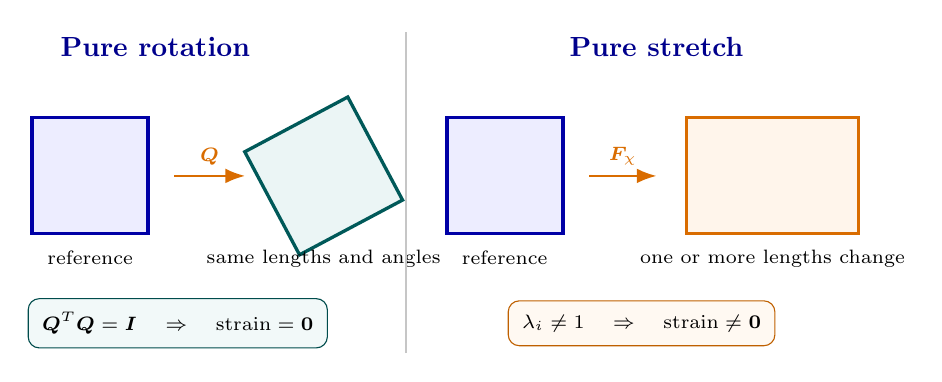
\begin{tikzpicture}[x=0.95cm,y=0.95cm,>=Latex,every node/.style={font=\scriptsize}]
  \node[font=\bfseries\normalsize,blue!55!black] at (-3.35,2.35) {Pure rotation};
  \fill[blue!7] (-5.0,-0.15) rectangle (-3.45,1.40);
  \draw[blue!65!black,very thick] (-5.0,-0.15) rectangle (-3.45,1.40);
  \node at (-4.22,-0.48) {reference};
  \draw[-{Latex[length=2.5mm]},thick,orange!85!black] (-3.10,0.62)--(-2.15,0.62)
    node[midway,above] {$\bm Q$};
  \begin{scope}[shift={(-1.1,0.62)},rotate=28]
    \fill[teal!8] (-0.78,-0.78) rectangle (0.78,0.78);
    \draw[teal!70!black,very thick] (-0.78,-0.78) rectangle (0.78,0.78);
  \end{scope}
  \node at (-1.10,-0.48) {same lengths and angles};
  \node[draw=teal!60!black,rounded corners,fill=teal!5,inner sep=5pt]
    at (-3.05,-1.35) {$\bm Q^T\bm Q=\I\quad\Rightarrow\quad\text{strain}=\bm0$};

  \draw[gray!45,line width=0.7pt] (0,-1.75)--(0,2.55);

  \node[font=\bfseries\normalsize,blue!55!black] at (3.35,2.35) {Pure stretch};
  \fill[blue!7] (0.55,-0.15) rectangle (2.10,1.40);
  \draw[blue!65!black,very thick] (0.55,-0.15) rectangle (2.10,1.40);
  \node at (1.32,-0.48) {reference};
  \draw[-{Latex[length=2.5mm]},thick,orange!85!black] (2.45,0.62)--(3.35,0.62)
    node[midway,above] {$\Fdef$};
  \fill[orange!8] (3.75,-0.15) rectangle (6.05,1.40);
  \draw[orange!85!black,very thick] (3.75,-0.15) rectangle (6.05,1.40);
  \node at (4.90,-0.48) {one or more lengths change};
  \node[draw=orange!75!black,rounded corners,fill=orange!5,inner sep=5pt]
    at (3.15,-1.35) {$\lambda_i\ne1\quad\Rightarrow\quad\text{strain}\ne\bm0$};
\end{tikzpicture}
\end{frame}

% ----- 23. Small strain -----
\begin{frame}{Displacement gradient and linearized strain}
With
\[
  \chi=\X+\bm{d},
  \qquad
  \Fdef=\I+\gradX\bm{d},
\]
the linearized strain is
\[
  \boxed{
  \bm{\varepsilon}
  =\operatorname{sym}(\gradX\bm{d})
  =\frac12\left(
    \gradX\bm{d}
    +(\gradX\bm{d})^T
  \right)
  }.
\]
\begin{punchbox}
\small
This approximation assumes small displacement gradients, including small rotations. Finite rotations require a nonlinear strain measure.
\end{punchbox}
\end{frame}

% ----- 24. C and B -----
\begin{frame}{Right and left Cauchy--Green tensors}
\begin{columns}[T,onlytextwidth]
\begin{column}{0.48\textwidth}
\[
  \Cten=\Fdef^T\Fdef
  \qquad\text{(material)}
\]
\[
  \Bten=\Fdef\Fdef^T
  \qquad\text{(spatial)}
\]
When \(J>0\), both are symmetric positive definite and share the eigenvalues \(\lambda_i^2\).
\end{column}
\begin{column}{0.50\textwidth}
\begin{punchbox}
\small
Under a superposed spatial rotation
\(\Fdef^\star=\bm{Q}\Fdef\),
\[
  \Cten^\star=\Cten,
  \qquad
  \Bten^\star=\bm{Q}\Bten\bm{Q}^T.
\]
\(\Cten\) remains unchanged. \(\Bten\) rotates with the spatial frame, while its scalar invariants remain unchanged.
\end{punchbox}
\end{column}
\end{columns}
\end{frame}

% ----- 25. E definition -----
\begin{frame}{Green--Lagrange strain}
\[
  \boxed{
  \Eten
  =\frac12(\Cten-\I)
  =\frac12(\Fdef^T\Fdef-\I)
  }.
\]
In components,
\[
  E_{IJ}
  =
  \frac12(C_{IJ}-\delta_{IJ}),
  \qquad
  C_{IJ}
  =
  \sum_{i=1}^{d}(F_\chi)_{iI}(F_\chi)_{iJ}.
\]
\begin{columns}[T,onlytextwidth]
\begin{column}{0.48\textwidth}
\textbf{Configuration}

\(\Eten\) acts on material line elements.
\end{column}
\begin{column}{0.50\textwidth}
\textbf{Small-deformation limit}

\(\Eten=\bm{\varepsilon}+O(\lVert\gradX\bm{d}\rVert^2)\).
\end{column}
\end{columns}
\end{frame}

% ----- 26. E geometry -----
\begin{frame}{Green--Lagrange strain and length change}
\begin{columns}[T,onlytextwidth]
\begin{column}{0.45\textwidth}
For a material line element,
\[
  d\x=\Fdef\,d\X.
\]
Then
\[
  \lVert d\x\rVert^2-\lVert d\X\rVert^2
  =
  2\,d\X\cdot\Eten\,d\X.
\]
\begin{punchbox}
\small
\(\Eten=\bm{0}\) means that local lengths are preserved. For a compatible deformation of a connected body, this corresponds to rigid motion.
\end{punchbox}
\end{column}
\begin{column}{0.55\textwidth}
\centering
\includegraphics[width=\linewidth]{pictures/4-2/Green-Lagrange.png}\\
\soft{\scriptsize The strain is expressed using the original material line element.}
\end{column}
\end{columns}
\end{frame}

% ----- 27. e definition -----
\begin{frame}{Euler--Almansi strain}
The spatial finite-strain measure is
\[
  \boxed{
  \eten
  =
  \frac12(\I-\Bten^{-1})
  =
  \frac12\left[
    \I-(\Fdef\Fdef^T)^{-1}
  \right]
  }.
\]
\begin{columns}[T,onlytextwidth]
\begin{column}{0.49\textwidth}
\textbf{Green--Lagrange}

\(\Eten\) acts on vectors in the reference configuration.
\end{column}
\begin{column}{0.49\textwidth}
\textbf{Euler--Almansi}

\(\eten\) acts on vectors in the current configuration.
\end{column}
\end{columns}
\begin{punchbox}
\small
IBFE derivations usually favor \(\Fdef\), \(\Cten\), and \(\Eten\) because finite-element integration occurs on \(B_0\).
\end{punchbox}
\end{frame}

% ----- 28. e geometry -----
\begin{frame}{Euler--Almansi strain and current line elements}
Take a current line element \(d\x\). Its material counterpart is
\[
  d\X=\Fdef^{-1}d\x.
\]
Therefore
\[
  \lVert d\x\rVert^2-\lVert d\X\rVert^2
  =
  d\x\cdot(\I-\Bten^{-1})d\x
  =
  2\,d\x\cdot\eten\,d\x.
\]
The two finite-strain measures are related by
\[
  \boxed{\eten=\Fdef^{-T}\Eten\Fdef^{-1}}.
\]
\begin{punchbox}
\small
The formulas describe the same deformation using different coordinates.
\end{punchbox}
\end{frame}

% ----- 29. Rotation check -----
\begin{frame}{Micro-check: pure rotation}
Let
\[
  \chi(\X)=\bm{Q}\X+\bm{c},
  \qquad
  \bm{Q}^T\bm{Q}=\I,
  \qquad
  \det\bm{Q}=1.
\]
Then
\[
  \Fdef=\bm{Q},
  \qquad
  \Cten=\bm{Q}^T\bm{Q}=\I,
  \qquad
  \Eten=\bm{0}.
\]
Also,
\[
  \Bten=\bm{Q}\bm{Q}^T=\I,
  \qquad
  \eten=\bm{0}.
\]
\begin{punchbox}
\small
Both finite-strain measures pass the rigid-rotation test.
\end{punchbox}
\end{frame}

% ----- 30. Shear check -----
\begin{frame}{Micro-check: simple shear}
For
\[
  \Fdef=
  \begin{bmatrix}
    1&\gamma&0\\
    0&1&0\\
    0&0&1
  \end{bmatrix},
\]
compute
\[
  \Cten=
  \begin{bmatrix}
    1&\gamma&0\\
    \gamma&1+\gamma^2&0\\
    0&0&1
  \end{bmatrix},
\qquad
  \Eten=
  \begin{bmatrix}
    0&\gamma/2&0\\
    \gamma/2&\gamma^2/2&0\\
    0&0&0
  \end{bmatrix}.
\]
\begin{punchbox}
\small
Linearized strain retains the terms proportional to \(\gamma\). Finite strain also contains the normal-strain term \(\gamma^2/2\).
\end{punchbox}
\end{frame}

% ----- 30a. Polar decomposition -----
\begin{frame}{Polar decomposition: \(\Fdef=\bm{R}\bm{U}=\bm{V}\bm{R}\)}
\small
Every deformation gradient with \(\det\Fdef>0\) factors \hi{uniquely} as
\[
  \boxed{\Fdef=\bm{R}\bm{U}=\bm{V}\bm{R}},
  \qquad
  \bm{R}^T\bm{R}=\I,
  \qquad
  \det\bm{R}=1,
\]
\[
  \bm{U}=\sqrt{\Fdef^T\Fdef}=\sqrt{\Cten},
  \qquad
  \bm{V}=\sqrt{\Fdef\Fdef^T}=\sqrt{\Bten},
  \qquad
  \bm{V}=\bm{R}\bm{U}\bm{R}^T .
\]
The right stretch \(\bm{U}\) and the left stretch \(\bm{V}\) are symmetric positive definite; \(\bm{R}\) is proper orthogonal.
\begin{columns}[T,onlytextwidth]
\begin{column}{0.47\textwidth}
\textbf{Reading \(\bm{R}\bm{U}\)}

Stretch first along the eigenvectors of \(\bm{U}\) by the principal stretches \(\lambda_i\), then rotate by \(\bm{R}\).
\end{column}
\begin{column}{0.49\textwidth}
\textbf{Reading \(\bm{V}\bm{R}\)}

Rotate first by the same \(\bm{R}\), then stretch by the same \(\lambda_i\) in the rotated frame.
\end{column}
\end{columns}
\smallskip

The eigenvalues of \(\bm{U}\) are the principal stretches \(\lambda_i\); the eigenvalues of \(\Cten=\bm{U}^2\) are \(\lambda_i^2\).
\begin{punchbox}
\footnotesize
\hi{Consequence.} Objectivity demands \(W(\bm{Q}\Fdef)=W(\Fdef)\) for every rotation \(\bm{Q}\). Take \(\bm{Q}=\bm{R}^T\):
\(W(\Fdef)=W(\bm{R}^T\bm{R}\bm{U})=W(\bm{U})=:\widehat W(\bm{U})=\widetilde W(\Cten)\).
A strain energy can see \(\Fdef\) only through \(\bm{U}\), equivalently through \(\Cten=\bm{U}^2\).
\end{punchbox}
\end{frame}

% ----- 30b. Polar decomposition: worked check -----
\begin{frame}{Polar decomposition: worked check}
\footnotesize
Take the simple shear of the previous slide in the \(X_1X_2\) plane with \(\gamma=1\):
\[
  \Fdef=
  \begin{bmatrix}1&\gamma\\0&1\end{bmatrix}
  =\begin{bmatrix}1&1\\0&1\end{bmatrix},
  \qquad
  \Cten=\Fdef^T\Fdef=
  \begin{bmatrix}1&\gamma\\\gamma&1+\gamma^2\end{bmatrix}
  =\begin{bmatrix}1&1\\1&2\end{bmatrix}.
\]
\textbf{Principal stretches.}
\(\lambda_{1,2}=\frac12\left(\sqrt{4+\gamma^2}\pm\gamma\right)\), so
\(\lambda_1=\frac{\sqrt5+1}{2}\approx1.618\),
\(\lambda_2=\frac{\sqrt5-1}{2}\approx0.618\),
and \(\lambda_1\lambda_2=1=\det\Fdef\).
The eigenvalues of \(\Cten\) are \(\lambda_1^2\approx2.618\) and \(\lambda_2^2\approx0.382\).
\[
  \bm{U}=\sqrt{\Cten}=\frac{1}{\sqrt5}
  \begin{bmatrix}2&1\\1&3\end{bmatrix}
  \approx
  \begin{bmatrix}0.894&0.447\\0.447&1.342\end{bmatrix},
  \qquad
  \bm{R}=\Fdef\bm{U}^{-1}=\frac{1}{\sqrt5}
  \begin{bmatrix}2&1\\-1&2\end{bmatrix}
  \approx
  \begin{bmatrix}0.894&0.447\\-0.447&0.894\end{bmatrix}.
\]
Checks: \(\bm{U}^2=\Cten\), \(\bm{R}^T\bm{R}=\I\), \(\det\bm{R}=1\), and \(\bm{R}\) is a clockwise rotation through \(\theta\) with \(\tan\theta=\gamma/2=\tfrac12\), that is \(\theta\approx26.6^\circ\).
\begin{punchbox}
\footnotesize
Simple shear is a stretch of \(\lambda_1\) along one principal direction, a compression \(\lambda_2=1/\lambda_1\) along the other, plus a rigid rotation by \(\theta\); that rotation is exactly what \(\Cten\) and \(\Eten\) discard.
\end{punchbox}
\end{frame}

% ----- 31. Invariants -----
\begin{frame}{Strain invariants and volume change}
In three dimensions,
\[
  I_1=\operatorname{tr}\Cten,
  \quad
  I_2=\frac12\left[
    (\operatorname{tr}\Cten)^2-\operatorname{tr}(\Cten^2)
  \right],
  \quad
  I_3=\det\Cten=J^2.
\]
\begin{columns}[T,onlytextwidth]
\begin{column}{0.48\textwidth}
\begin{block}{Raw invariants}
\(I_1\) and \(I_2\) respond to both shape change and volume change. \(I_3\) measures volume change directly.
\end{block}
\end{column}
\begin{column}{0.50\textwidth}
\begin{block}{Isochoric invariants}
Using \(\bar{\Fdef}=J^{-1/3}\Fdef\) and
\(\bar{\Cten}=\bar{\Fdef}^T\bar{\Fdef}\),
\[
  \bar I_1=\operatorname{tr}\bar{\Cten},
  \qquad
  \bar I_2=\tfrac12[
    (\operatorname{tr}\bar{\Cten})^2
    -\operatorname{tr}(\bar{\Cten}^2)] .
\]
\end{block}
\end{column}
\end{columns}
\end{frame}

% ----- 32. Module 2 wrap -----
\begin{frame}{Module 2 wrap-up}
\begin{itemize}\itemsep6pt
  \item \(\gradX\bm{d}=\Fdef-\I\) is the displacement gradient.
  \item \(\Cten=\Fdef^T\Fdef\) and \(\Bten=\Fdef\Fdef^T\) encode stretch.
  \item \(\Eten=\tfrac12(\Cten-\I)\) is a material finite-strain measure.
  \item \(\eten=\tfrac12(\I-\Bten^{-1})\) is its spatial counterpart.
  \item \(I_3=J^2\). Modified invariants isolate isochoric deformation.
\end{itemize}
\begin{punchbox}
\small
Quick check: \(J=1\) implies \(I_3=1\), but it does not imply \(\Eten=\bm{0}\).
\end{punchbox}
\end{frame}

\section{Stress measures and transformations}

% ----- 33. Module 3 -----
\begin{frame}{Module 3: why several stress measures?}
Fluid mechanics normally uses the Cauchy stress
\[
  \sigmaC(\x,t)
\]
in the current configuration. IBFE constitutive calculations usually use reference coordinates and the stresses
\[
  \Pten(\X,t)
  \qquad\text{and}\qquad
  \Sten(\X,t).
\]
\begin{punchbox}
\small
Each stress measure pairs with a particular normal, area measure, or deformation rate. Conversions between them describe the same physical force or power.
\end{punchbox}
\end{frame}

% ----- 34. Cauchy stress -----
\begin{frame}{Cauchy stress and current traction}
For a current surface with outward unit normal \(\nvec\),
\[
  \boxed{\tvec(\nvec)=\sigmaC\,\nvec}.
\]
The differential force acting on current area \(da\) is
\[
  d\bm{f}
  =
  \sigmaC\,\nvec\,da.
\]
In components,
\[
  t_i=\sigma_{ij}n_j.
\]
\begin{punchbox}
\small
The Cauchy stress maps a current normal to force per current area. Its diagonal entries describe normal stress and its off-diagonal entries describe shear stress in the chosen basis.
\end{punchbox}
\end{frame}

% ----- 35. Traction figure -----
\begin{frame}{Traction vectors on coordinate planes}
\begin{columns}[T,onlytextwidth]
\begin{column}{0.35\textwidth}
\[
  \tvec(\nvec)=\sigmaC\nvec.
\]
Choosing each coordinate normal selects one column of the Cauchy-stress matrix.

\medskip
For example,
\[
  \tvec(\bm{e}_1)
  =
  \begin{bmatrix}
    \sigma_{11}\\
    \sigma_{21}\\
    \sigma_{31}
  \end{bmatrix}.
\]
\end{column}
\begin{column}{0.65\textwidth}
\centering
\includegraphics[width=0.74\linewidth]{pictures/4-2/traction-vectors.png}

{\tiny Source: P.~A. Kelly, \emph{Solid Mechanics Part III: Foundations of Continuum Solid Mechanics}, \S3.3, Fig.~3.3.2 (University of Auckland lecture notes, \url{https://pkel015.connect.amazon.auckland.ac.nz/SolidMechanicsBooks/}). The figure's equation numbers refer to those notes.}
\end{column}
\end{columns}
\end{frame}

% ----- 36. PK1 -----
\begin{frame}{First Piola--Kirchhoff stress}
The first Piola stress is a two-point tensor defined on \(B_0\):
\[
  \Pten(\X,t)\in\R^{d\times d}.
\]
For a reference surface with outward unit normal \(\Nvec\) and reference area \(dA\),
\[
  \boxed{d\bm{f}=\Pten\Nvec\,dA}.
\]
Thus
\[
  \bm{t}_0(\Nvec)=\Pten\Nvec
\]
is force per reference area, directed in the current configuration.
\begin{punchbox}
\small
\(\Pten\) is generally nonsymmetric because its two indices refer to different configurations.
\end{punchbox}
\end{frame}

% ----- 37. Matching patches -----
\begin{frame}{Matching reference and current surface patches}
\begin{columns}[T,onlytextwidth]
\begin{column}{0.46\textwidth}
The same physical force can be described on corresponding patches:
\[
  d\bm{f}
  =
  \sigmaC\nvec\,da
  =
  \Pten\Nvec\,dA.
\]
\begin{itemize}\itemsep5pt
  \item \(\sigmaC\nvec\): force per current area
  \item \(\Pten\Nvec\): force per reference area
\end{itemize}
\begin{punchbox}
\small
The area vectors differ. Nanson's formula supplies the missing geometric transformation.
\end{punchbox}
\end{column}
\begin{column}{0.54\textwidth}
\centering
\includegraphics[width=\linewidth]{pictures/4-2/traction-vectors-B0-B1.png}

{\scriptsize Source: Kelly, \emph{Solid Mechanics Part III}, \S3.5, Fig.~3.5.1 (same notes). NB: the figure labels the reference traction \(\bm{PN}\) as \(\bm{T}\); in this course that quantity is \(\bm{t}_0\), and \(\bm{T}\) is reserved for the transmission force \(-\bm{PN}\).}
\end{column}
\end{columns}
\end{frame}

% ----- 38. Nanson -----
\begin{frame}{Nanson's formula}
Corresponding oriented area elements satisfy
\[
  \boxed{
  \nvec\,da
  =
  J\,\Fdef^{-T}\Nvec\,dA
  }.
\]
\begin{columns}[T,onlytextwidth]
\begin{column}{0.49\textwidth}
\textbf{Reference area vector}
\[
  \Nvec\,dA
\]
uses the material normal and reference area.
\end{column}
\begin{column}{0.49\textwidth}
\textbf{Current area vector}
\[
  \nvec\,da
\]
uses the spatial normal and current area.
\end{column}
\end{columns}
\begin{punchbox}
\small
In three dimensions, the identity follows by transforming two tangent vectors and using
\[
  (\Fdef\bm{a})\times(\Fdef\bm{b})
  =
  J\Fdef^{-T}(\bm{a}\times\bm{b}).
\]
\end{punchbox}
\end{frame}

% ----- 39. Piola transform -----
\begin{frame}{Piola transformation}
Start from equality of force on matching patches:
\[
  \sigmaC\nvec\,da
  =
  \Pten\Nvec\,dA.
\]
Insert Nanson's formula:
\[
  \sigmaC
  \left(J\Fdef^{-T}\Nvec\,dA\right)
  =
  \Pten\Nvec\,dA.
\]
Because the relation holds for every \(\Nvec\),
\[
  \boxed{\Pten=J\,\sigmaC\,\Fdef^{-T}}.
\]
Equivalently,
\[
  \boxed{\sigmaC=J^{-1}\Pten\Fdef^T}.
\]
\end{frame}

% ----- 40. PK2 -----
\begin{frame}{Second Piola--Kirchhoff stress}
Pull the remaining spatial index of \(\Pten\) back to the reference configuration:
\[
  \boxed{
  \Sten=\Fdef^{-1}\Pten
  },
\qquad
  \boxed{
  \Pten=\Fdef\Sten
  }.
\]
\begin{columns}[T,onlytextwidth]
\begin{column}{0.49\textwidth}
\begin{block}{Configuration}
\(\Sten\) has two material indices and acts entirely in the reference description.
\end{block}
\end{column}
\begin{column}{0.49\textwidth}
\begin{block}{Energy pairing}
\[
  \Pten:\dot{\Fdef}
  =
  \frac12\Sten:\dot{\Cten}.
\]
\end{block}
\end{column}
\end{columns}
\begin{punchbox}
\small
If the Cauchy stress is symmetric, then \(\Sten\) is symmetric.
\end{punchbox}
\end{frame}

% ----- 41. Checks -----
\begin{frame}{Dimensional, symmetry, and power checks}
\small
\begin{center}
\renewcommand{\arraystretch}{1.18}
\begin{tabular}{llll}
\toprule
Measure & Area basis & Symmetry & Power pairing \\
\midrule
\(\sigmaC\) & current & symmetric$^\ast$ & \(J\sigmaC:\bm{D}\) \\
\(\Pten\) & reference & generally no & \(\Pten:\dot{\Fdef}\) \\
\(\Sten\) & reference & symmetric$^\ast$ & \(\tfrac12\Sten:\dot{\Cten}\) \\
\bottomrule
\end{tabular}
\end{center}
\[
  \Pten:\dot{\Fdef}
  =
  \frac12\Sten:\dot{\Cten}
  =
  J\,\sigmaC:\bm{D},
\qquad
  \bm{D}=\operatorname{sym}(\gradx\uEuler).
\]
\begin{punchbox}
\small
\({}^\ast\)Symmetry follows for a classical nonpolar continuum satisfying angular-momentum balance.
\end{punchbox}
\end{frame}

% ----- 42. Module 3 wrap -----
\begin{frame}{Module 3 wrap-up}
\begin{itemize}\itemsep6pt
  \item Current traction: \(\tvec=\sigmaC\nvec\).
  \item Reference traction: \(\bm{t}_0=\Pten\Nvec\).
  \item Oriented areas:
  \[
    \nvec\,da=J\Fdef^{-T}\Nvec\,dA.
  \]
  \item Stress conversions:
  \[
    \Pten=J\sigmaC\Fdef^{-T},
    \qquad
    \sigmaC=J^{-1}\Pten\Fdef^T,
    \qquad
    \Sten=\Fdef^{-1}\Pten.
  \]
\end{itemize}
\begin{punchbox}
\small
The normal, area measure, and stress tensor must belong to matching configurations.
\end{punchbox}
\end{frame}

% ----- 43. IBFE bridge -----
\begin{frame}{IBFE notation bridge}
\small
\begin{center}
\renewcommand{\arraystretch}{1.2}
\begin{tabular}{lll}
\toprule
Object & Symbol here & Role in IBFE \\
\midrule
Deformation gradient & \(\Fdef=\gradX\chi\) & structural kinematics \\
First Piola stress & \(\Pten\) & constitutive response \\
Lagrangian force & \(\FLag\) & weak structural force \\
Eulerian force & \(\fEuler\) & fluid momentum source \\
Cauchy stress & \(\sigmaC\) & current-configuration stress \\
\bottomrule
\end{tabular}
\end{center}
\begin{punchbox}
\centering
\[
  W(\Fdef)
  \longrightarrow
  \Pten
  \longrightarrow
  \FLag
  \longrightarrow
  \fEuler .
\]
\end{punchbox}
\end{frame}

\section{Hyperelasticity and IBFE force construction}

% ----- 44. Module 4 -----
\begin{frame}{Module 4: hyperelasticity}
A hyperelastic material stores energy according to a scalar density per reference volume:
\[
  W:\R^{d\times d}\to\R,
  \qquad
  \Fdef\mapsto W(\Fdef).
\]
The first Piola stress follows by differentiation:
\[
  \boxed{
  \Pten=\frac{\partial W}{\partial\Fdef}
  }.
\]
\begin{punchbox}
\small
One scalar function encodes the constitutive response. Differentiating once gives stress. Differentiating again gives the material tangent used in nonlinear solvers.
\end{punchbox}
\end{frame}

% ----- 45. Matrix derivative -----
\begin{frame}{Derivative of a scalar with respect to a matrix}
The derivative has the same tensor shape as its matrix argument:
\[
  \left(
  \frac{\partial W}{\partial\Fdef}
  \right)_{iI}
  :=
  \frac{\partial W}{\partial(F_\chi)_{iI}}.
\]
In three dimensions,
\[
  \frac{\partial W}{\partial\Fdef}
  =
  \begin{bmatrix}
  \dfrac{\partial W}{\partial(F_\chi)_{11}}&
  \dfrac{\partial W}{\partial(F_\chi)_{12}}&
  \dfrac{\partial W}{\partial(F_\chi)_{13}}\\[6pt]
  \dfrac{\partial W}{\partial(F_\chi)_{21}}&
  \dfrac{\partial W}{\partial(F_\chi)_{22}}&
  \dfrac{\partial W}{\partial(F_\chi)_{23}}\\[6pt]
  \dfrac{\partial W}{\partial(F_\chi)_{31}}&
  \dfrac{\partial W}{\partial(F_\chi)_{32}}&
  \dfrac{\partial W}{\partial(F_\chi)_{33}}
  \end{bmatrix}.
\]
\begin{punchbox}
\small
Shape check: \(W\) is scalar, while
\(\partial W/\partial\Fdef\in\R^{d\times d}\).
\end{punchbox}
\end{frame}

% ----- 46. Directional derivative -----
\begin{frame}{Directional derivative and double contraction}
Perturb \(\Fdef\) in an arbitrary direction \(\delta\Fdef\):
\[
  \delta W
  :=
  \left.
  \frac{d}{d\varepsilon}
  W(\Fdef+\varepsilon\,\delta\Fdef)
  \right|_{\varepsilon=0}.
\]
The matrix derivative is defined by
\[
  \boxed{
  \delta W
  =
  \frac{\partial W}{\partial\Fdef}:\delta\Fdef
  =
  \Pten:\delta\Fdef
  }.
\]
The double contraction is the Frobenius inner product:
\[
  \bm{A}:\bm{B}
  =
  \sum_{i,I}A_{iI}B_{iI}
  =
  \operatorname{tr}(\bm{A}^T\bm{B}).
\]
\end{frame}

% ----- 47. Objectivity and isotropy -----
\begin{frame}{Objectivity and isotropy}
\begin{columns}[T,onlytextwidth]
\begin{column}{0.49\textwidth}
\begin{block}{Frame indifference}
For every proper orthogonal spatial rotation \(\bm{Q}\),
\[
  W(\bm{Q}\Fdef)=W(\Fdef).
\]
An objective energy may be written in terms of
\(\Cten=\Fdef^T\Fdef\).
\end{block}
\end{column}
\begin{column}{0.49\textwidth}
\begin{block}{Material isotropy}
For every proper orthogonal material rotation \(\bm{R}\),
\[
  W(\Fdef\bm{R})=W(\Fdef).
\]
An objective isotropic energy may be written using the invariants of \(\Cten\).
\end{block}
\end{column}
\end{columns}
\begin{punchbox}
\small
An anisotropic material can remain objective. Its energy also depends on material directions or structural tensors.
\end{punchbox}
\end{frame}

% ----- 48. Compressibility -----
\begin{frame}{Compressible and incompressible response}
\small
\begin{columns}[T,onlytextwidth]
\begin{column}{0.49\textwidth}
\begin{block}{Exact incompressibility}
\[
  J=1
\]
is a constraint. A pressure-like Lagrange multiplier contributes
\[
  -p_s\,J\Fdef^{-T}
\]
to the first Piola stress.
\end{block}
\end{column}
\begin{column}{0.49\textwidth}
\begin{block}{Nearly incompressible model}
\[
  W(\Fdef)
  =
  W_{\mathrm{iso}}(\bar{\Fdef})+U(J)
\]
uses a volumetric energy to discourage numerical volume change.
\end{block}
\end{column}
\end{columns}
\[
  \dot J
  =
  J\,(\divx\uEuler)\circ\chi .
\]
\begin{punchbox}
\small
At the continuum level, no slip and \(\divx\uEuler=0\) preserve the initial value \(J(\X,0)\). They give \(J\equiv1\) only when \(J(\X,0)=1\). Discrete IBFE solutions can still develop local volume error.
\end{punchbox}
\end{frame}

% ----- 49. Isochoric split -----
\begin{frame}{Isochoric and volumetric deformation}
In spatial dimension \(d\), define
\[
  \boxed{
  \bar{\Fdef}=J^{-1/d}\Fdef
  },
\qquad
  \det\bar{\Fdef}=1.
\]
Then
\[
  \bar{\Cten}
  =
  \bar{\Fdef}^T\bar{\Fdef},
\]
and the modified invariants of \(\bar{\Cten}\) describe the isochoric response.
\begin{columns}[T,onlytextwidth]
\begin{column}{0.49\textwidth}
\[
  \bar{\Fdef}=J^{-1/2}\Fdef
  \quad\text{in 2D},
\]
\end{column}
\begin{column}{0.49\textwidth}
\[
  \bar{\Fdef}=J^{-1/3}\Fdef
  \quad\text{in 3D}.
\]
\end{column}
\end{columns}

\smallskip
Equivalently, in 3D the motion splits multiplicatively into a volumetric and a distortional part,
\[
  \Fdef=J^{1/3}\bar{\Fdef},
  \qquad
  \bar{\Fdef}=J^{-1/3}\Fdef .
\]
\begin{punchbox}
\small
Building the distortional energy from modified invariants prevents the shear response from also penalizing volume change.

\smallskip
{\scriptsize Griffith \& Patankar (2020, \S2.2.2) report that modified invariants together with volumetric stabilization give accuracy comparable to stabilized finite-element formulations on the Bonet et al.\ (2015) twisted-beam benchmark.}
\end{punchbox}
\end{frame}

% ----- 50. Volumetric penalty -----
\begin{frame}{Volumetric stabilization}
\begin{columns}[T,onlytextwidth]
\begin{column}{0.44\textwidth}
A common positive-\(J\) choice is
\[
  U(J)
  =
  \frac{\kappa_{\mathrm{stab}}}{2}
  (\ln J)^2.
\]
It satisfies
\[
  U(1)=0,
  \qquad
  U'(1)=0.
\]
{\scriptsize Unlike a quadratic \((J-1)^2\) penalty, \((\ln J)^2\) diverges as \(J\to0^+\): the barrier shown in the plot.}

Its Piola-stress contribution is
\[
  \Pten_{\mathrm{vol}}
  =
  U'(J)J\Fdef^{-T}
  =
  \kappa_{\mathrm{stab}}\ln J\,\Fdef^{-T}.
\]
\end{column}
\begin{column}{0.56\textwidth}
\centering
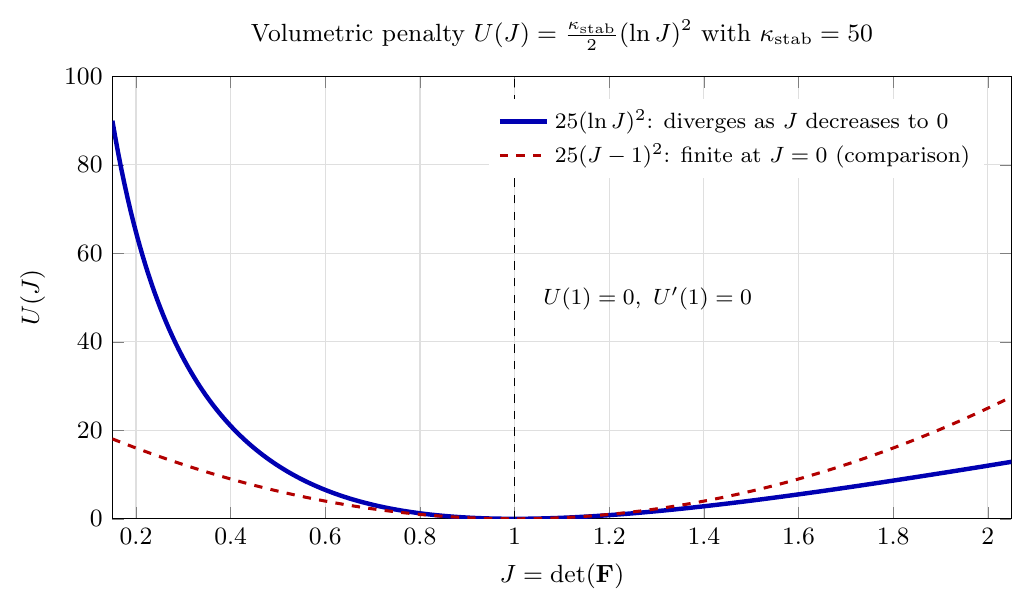
\includegraphics[width=\linewidth]{pictures/4-2/Wvol_J_plot.png}
\end{column}
\end{columns}
\begin{punchbox}
\scriptsize
In an incompressible IBFE model, \(\kappa_{\mathrm{stab}}\) controls numerical volume error. It need not equal a physical bulk modulus.
\end{punchbox}
\end{frame}

% ----- 51. Neo-Hookean energy -----
\begin{frame}{Compressible neo-Hookean energy}
One common three-dimensional model is
\[
  \boxed{
  W(\Fdef)
  =
  \frac{\mu}{2}(I_1-3)
  -\mu\ln J
  +\frac{\lambda_{\mathrm L}}{2}(\ln J)^2
  },
\]
where
\[
  I_1=\operatorname{tr}(\Fdef^T\Fdef),
  \qquad
  J=\det\Fdef>0.
\]
\begin{itemize}\itemsep5pt
  \item \(\mu\) is the infinitesimal shear modulus.
  \item \(\lambda_{\mathrm L}\) is the first Lamé parameter.
  \item The infinitesimal bulk modulus is
  \(K=\lambda_{\mathrm L}+2\mu/3\).
\end{itemize}
\begin{punchbox}
\small
This distinction keeps a material Lamé parameter separate from the optional stabilization coefficient \(\kappa_{\mathrm{stab}}\). In an (nearly) incompressible IBFE model, the \((\ln J)^2\) term of the neo-Hookean \(W\) plays exactly the role of \(\kappa_{\mathrm{stab}}\).
\end{punchbox}
\end{frame}

% ----- 52. Closed P -----
\begin{frame}{Neo-Hookean first Piola stress}
For the energy on the previous slide,
\[
  \boxed{
  \Pten
  =
  \mu\left(\Fdef-\Fdef^{-T}\right)
  +\lambda_{\mathrm L}\ln J\,\Fdef^{-T}
  }.
\]
\begin{columns}[T,onlytextwidth]
\begin{column}{0.48\textwidth}
\begin{block}{Reference state}
At \(\Fdef=\I\),
\[
  J=1,
  \qquad
  \Pten=\bm{0}.
\]
\end{block}
\end{column}
\begin{column}{0.48\textwidth}
\begin{block}{Isochoric state}
If \(J=1\),
\[
  \Pten
  =
  \mu(\Fdef-\Fdef^{-T}).
\]
\end{block}
\end{column}
\end{columns}
\begin{punchbox}
\small
The final section derives this expression term by term.
\end{punchbox}
\end{frame}

% ----- 53. Stress conversions -----
\begin{frame}{Neo-Hookean stress conversions}
Once \(\Pten\) is known,
\[
  \Sten=\Fdef^{-1}\Pten,
  \qquad
  \sigmaC=J^{-1}\Pten\Fdef^T.
\]
For the compressible neo-Hookean model,
\[
  \boxed{
  \sigmaC
  =
  \frac{\mu}{J}(\Bten-\I)
  +\frac{\lambda_{\mathrm L}\ln J}{J}\I
  }.
\]
\begin{punchbox}
\small
\(\sigmaC\) is symmetric because \(\Bten\) and \(\I\) are symmetric. The same constitutive response appears different because each stress uses a different configuration and area measure.
\end{punchbox}
\end{frame}

% ----- 54. Pipeline -----
\begin{frame}{IBFE force pipeline}
\small
\begin{enumerate}\itemsep5pt
  \item Evaluate \({\Fdef}_h=\gradX\chi_h\), \(J_h\), and
  \(\Pten_h=\partial W/\partial\Fdef\) at structural quadrature points.
  \item Define the unified Lagrangian force by negative virtual work:
  \[
    \int_{B_0}\FLag_h\cdot\bm{V}_h\,dV
    =
    -\int_{B_0}\Pten_h:\gradX\bm{V}_h\,dV.
  \]
  \item Spread \(\FLag_h\) to the Eulerian grid with a regularized delta kernel.
  \item Advance the incompressible fluid equations.
  \item Restrict the Eulerian velocity back to the structure and update \(\chi_h\).
\end{enumerate}
\begin{punchbox}
\small
The negative sign makes internal elastic force oppose increasing stored energy. Prescribed body forces or boundary tractions add their own virtual-work terms.
\end{punchbox}
\end{frame}

% ----- 55. FE interpolation -----
\begin{frame}{Finite-element interpolation of motion and stress}
With structural basis functions \(\{\phi_\ell(\X)\}\),
\[
  \chi_h(\X,t)
  =
  \sum_{\ell=1}^{M}
  \chi_\ell(t)\phi_\ell(\X),
\]
\[
{\Fdef}_h(\X,t)
  =
  \sum_{\ell=1}^{M}
  \chi_\ell(t)\otimes\gradX\phi_\ell(\X).
\]
\begin{itemize}\itemsep5pt
  \item \(C^0\) interpolation makes \(\chi_h\) continuous.
  \item \({\Fdef}_h\) and \(\Pten_h\) are generally discontinuous across element boundaries.
  \item Constitutive stress and interaction forces are evaluated at element quadrature points.
  \item Interaction quadrature may be refined independently of structural nodes and helps prevent leakage when adequately resolved.
\end{itemize}
\end{frame}

% ----- 56. Module 4 wrap -----
\begin{frame}{Module 4 wrap-up}
\begin{itemize}\itemsep6pt
  \item Hyperelasticity defines \(\Pten=\partial W/\partial\Fdef\).
  \item The identity \(\delta W=\Pten:\delta\Fdef\) defines the matrix derivative.
  \item Objectivity and isotropy impose different constitutive requirements.
  \item Modified invariants and \(U(J)\) separate shape and volume response.
  \item The weak structural force carries a negative virtual-work sign.
  \item FE quadrature connects piecewise constitutive fields to the Eulerian grid.
\end{itemize}
\begin{punchbox}
\small
Next, one homogeneous deformation will pass through the entire chain from \(\chi\) to \(\sigmaC\).
\end{punchbox}
\end{frame}

\section{Worked example: uniaxial stretch (prescribed axial deformation)}

% ----- 57. Axial setup -----
\begin{frame}{Worked example: uniaxial stretch (prescribed axial deformation)}
Consider the three-dimensional motion
\[
  \chi(\X)
  =
  \begin{bmatrix}
    \alpha X_1\\
    X_2\\
    X_3
  \end{bmatrix},
  \qquad
  \alpha>0.
\]
\begin{itemize}\itemsep6pt
  \item Material points stretch by the factor \(\alpha\) along \(X_1\).
  \item The transverse coordinates remain unchanged.
  \item There is no shear.
\end{itemize}
\begin{punchbox}
\small
Throughout the course this example is called \emph{uniaxial stretch (prescribed axial deformation)}; it is sometimes also called uniaxial strain. It is not automatically a uniaxial-stress test because the lateral stretches are fixed.
\end{punchbox}
\end{frame}

% ----- 58. Axial F and J -----
\begin{frame}{Axial deformation gradient and Jacobian}
Differentiate each component of the motion:
\[
  \Fdef
  =
  \gradX\chi
  =
  \begin{bmatrix}
  \dfrac{\partial\chi_1}{\partial X_1}&
  \dfrac{\partial\chi_1}{\partial X_2}&
  \dfrac{\partial\chi_1}{\partial X_3}\\[5pt]
  \dfrac{\partial\chi_2}{\partial X_1}&
  \dfrac{\partial\chi_2}{\partial X_2}&
  \dfrac{\partial\chi_2}{\partial X_3}\\[5pt]
  \dfrac{\partial\chi_3}{\partial X_1}&
  \dfrac{\partial\chi_3}{\partial X_2}&
  \dfrac{\partial\chi_3}{\partial X_3}
  \end{bmatrix}
  =
  \operatorname{diag}(\alpha,1,1).
\]
Therefore
\[
  \boxed{J=\det\Fdef=\alpha}.
\]
\begin{punchbox}
\small
The prescribed deformation changes volume whenever \(\alpha\ne1\).
\end{punchbox}
\end{frame}

% ----- 59. Axial C and E -----
\begin{frame}{Axial Cauchy--Green tensor and Green strain}
Because \(\Fdef\) is diagonal,
\[
  \Cten
  =
  \Fdef^T\Fdef
  =
  \operatorname{diag}(\alpha^2,1,1).
\]
Then
\[
  \Eten
  =
  \frac12(\Cten-\I)
  =
  \operatorname{diag}\left(
    \frac{\alpha^2-1}{2},0,0
  \right).
\]
\begin{columns}[T,onlytextwidth]
\begin{column}{0.49\textwidth}
\[
  E_{11}=\frac{\alpha^2-1}{2}.
\]
\end{column}
\begin{column}{0.49\textwidth}
\[
  E_{22}=E_{33}=0.
\]
\end{column}
\end{columns}
\begin{punchbox}
\small
For \(\alpha=1+\varepsilon\) with \(|\varepsilon|\ll1\), \(E_{11}=\varepsilon+O(\varepsilon^2)\).
\end{punchbox}
\end{frame}

% ----- 60. Axial invariants -----
\begin{frame}{Axial-deformation invariants}
For
\[
  \Cten=\operatorname{diag}(\alpha^2,1,1),
\]
the first and third invariants are
\[
  I_1=\operatorname{tr}\Cten=\alpha^2+2,
\]
\[
  I_3=\det\Cten=\alpha^2=J^2.
\]
The second invariant is
\[
  I_2=1+2\alpha^2.
\]
\begin{punchbox}
\small
\(I_3\) directly records volume change. The raw invariants \(I_1\) and \(I_2\) reflect both the axial shape change and the accompanying volume change.
\end{punchbox}
\end{frame}

% ----- 61. Axial energy -----
\begin{frame}{Constitutive choice for the axial example}
Use the compressible neo-Hookean energy
\[
  W(\Fdef)
  =
  \frac{\mu}{2}(I_1-3)
  -\mu\ln J
  +\frac{\lambda_{\mathrm L}}{2}(\ln J)^2.
\]
For the prescribed axial deformation,
\[
  I_1=\alpha^2+2,
  \qquad
  J=\alpha,
\]
so
\[
  W(\alpha)
  =
  \frac{\mu}{2}(\alpha^2-1)
  -\mu\ln\alpha
  +\frac{\lambda_{\mathrm L}}{2}(\ln\alpha)^2.
\]
\begin{punchbox}
\small
The stress still follows by differentiating the full matrix-valued argument \(\Fdef\), not only the reduced scalar expression \(W(\alpha)\).
\end{punchbox}
\end{frame}

% ----- 62. Axial P -----
\begin{frame}{First Piola stress for the axial deformation}
Use
\[
  \Pten
  =
  \mu(\Fdef-\Fdef^{-T})
  +\lambda_{\mathrm L}\ln J\,\Fdef^{-T}.
\]
Here
\[
  \Fdef^{-T}
  =
  \operatorname{diag}(\alpha^{-1},1,1),
  \qquad
  \ln J=\ln\alpha.
\]
Therefore
\[
  \boxed{
  \Pten
  =
  \operatorname{diag}\left(
  \mu(\alpha-\alpha^{-1})
  +\lambda_{\mathrm L}\frac{\ln\alpha}{\alpha},
  \lambda_{\mathrm L}\ln\alpha,
  \lambda_{\mathrm L}\ln\alpha
  \right)
  }.
\]
\begin{punchbox}
\small
Fixing both lateral stretches to one generally produces nonzero transverse stress.
\end{punchbox}
\end{frame}

% ----- 63. Axial sigma -----
\begin{frame}{Cauchy stress for the axial deformation}
Use the Piola transformation:
\[
  \sigmaC
  =
  \frac{1}{J}\Pten\Fdef^T.
\]
Since \(J=\alpha\) and both tensors are diagonal,
\[
  \sigmaC
  =
  \operatorname{diag}\left(
    P_{11},
    \frac{P_{22}}{\alpha},
    \frac{P_{33}}{\alpha}
  \right).
\]
Thus
\[
  \sigma_{22}=\sigma_{33}
  =
  \frac{\lambda_{\mathrm L}\ln\alpha}{\alpha}.
\]
\begin{punchbox}
\small
A traction-free uniaxial-stress test must allow unknown lateral stretches and solve for them from \(\sigma_{22}=\sigma_{33}=0\).
\end{punchbox}
\end{frame}

% ----- 64. Axial wrap -----
\begin{frame}{Axial-example wrap-up}
\[
  \chi(\X)
  \longrightarrow
  \Fdef=\operatorname{diag}(\alpha,1,1)
  \longrightarrow
  J=\alpha
\]
\[
  \longrightarrow
  \Cten=\operatorname{diag}(\alpha^2,1,1)
  \longrightarrow
  \Eten=\frac12\operatorname{diag}(\alpha^2-1,0,0).
\]
After choosing \(W\),
\[
  W(\Fdef)
  \longrightarrow
  \Pten=\frac{\partial W}{\partial\Fdef}
  \longrightarrow
  \sigmaC=J^{-1}\Pten\Fdef^T.
\]
\begin{punchbox}
\small
Every arrow can be checked independently. Homogeneous deformations are useful unit tests for constitutive implementations.
\end{punchbox}
\end{frame}

\section{Neo-Hookean stress derivation}

% ----- 65. Derivation goal -----
\begin{frame}{Derivation goal}
Start with
\[
  W(\Fdef)
  =
  \frac{\mu}{2}(I_1-3)
  -\mu\ln J
  +\frac{\lambda_{\mathrm L}}{2}(\ln J)^2.
\]
We will compute the first variation and match
\[
  \delta W=\Pten:\delta\Fdef.
\]
Two identities drive the calculation:
\[
  \delta I_1
  =
  2\Fdef:\delta\Fdef,
  \qquad
  \delta(\ln J)
  =
  \Fdef^{-T}:\delta\Fdef.
\]
\begin{punchbox}
\small
The next two slides derive these identities before the terms are combined.
\end{punchbox}
\end{frame}

% ----- 66. Variation I1 -----
\begin{frame}{Step 1: variation of \(I_1\)}
Because
\[
  I_1
  =
  \operatorname{tr}(\Fdef^T\Fdef)
  =
  \sum_{i,I}(F_\chi)_{iI}^2,
\]
\[
  \delta I_1
  =
  2\sum_{i,I}
  (F_\chi)_{iI}\,
  \delta(F_\chi)_{iI}
  =
  \boxed{
  2\Fdef:\delta\Fdef
  }.
\]
Therefore
\[
  \delta\left[
  \frac{\mu}{2}(I_1-3)
  \right]
  =
  \mu\Fdef:\delta\Fdef.
\]
\begin{punchbox}
\small
This term contributes \(\mu\Fdef\) to \(\Pten\).
\end{punchbox}
\end{frame}

% ----- 67. Variation log J -----
\begin{frame}{Step 2: variation of \(\ln J\)}
Jacobi's determinant identity gives
\[
  \delta J
  =
  J\,\Fdef^{-T}:\delta\Fdef.
\]
The chain rule then gives
\[
  \boxed{
  \delta(\ln J)
  =
  \frac{\delta J}{J}
  =
  \Fdef^{-T}:\delta\Fdef
  }.
\]
Consequently,
\[
  \delta(-\mu\ln J)
  =
  -\mu\Fdef^{-T}:\delta\Fdef,
\]
\[
  \delta\left[
  \frac{\lambda_{\mathrm L}}{2}(\ln J)^2
  \right]
  =
  \lambda_{\mathrm L}\ln J\,
  \Fdef^{-T}:\delta\Fdef.
\]
\end{frame}

% ----- 68. Combine -----
\begin{frame}{Step 3: combine the stress contributions}
Collect the coefficients of \(\delta\Fdef\):
\[
  \delta W
  =
  \left[
    \mu\Fdef
    -\mu\Fdef^{-T}
    +\lambda_{\mathrm L}\ln J\,\Fdef^{-T}
  \right]
  :\delta\Fdef.
\]
Matching \(\delta W=\Pten:\delta\Fdef\) gives
\[
  \boxed{
  \Pten
  =
  \mu(\Fdef-\Fdef^{-T})
  +\lambda_{\mathrm L}\ln J\,\Fdef^{-T}
  }.
\]
\begin{columns}[T,onlytextwidth]
\begin{column}{0.49\textwidth}
\[
  \Fdef=\I
  \quad\Rightarrow\quad
  \Pten=\bm{0}.
\]
\end{column}
\begin{column}{0.49\textwidth}
\[
  J=1
  \quad\Rightarrow\quad
  \Pten=\mu(\Fdef-\Fdef^{-T}).
\]
\end{column}
\end{columns}
\end{frame}

% ----- 69. Small-strain check -----
\begin{frame}{Micro-check: small-strain limit}
Let
\[
  \Fdef=\I+\bm{H},
  \qquad
  \lVert\bm{H}\rVert\ll1,
  \qquad
  \bm{\varepsilon}=\operatorname{sym}\bm{H}.
\]
To first order,
\[
  \Fdef^{-T}\approx\I-\bm{H}^T,
  \qquad
  \ln J\approx\operatorname{tr}\bm{H}.
\]
Substitution gives
\[
  \Pten
  \approx
  \mu(\bm{H}+\bm{H}^T)
  +\lambda_{\mathrm L}\operatorname{tr}(\bm{H})\I
  =
  \boxed{
  2\mu\bm{\varepsilon}
  +\lambda_{\mathrm L}
  \operatorname{tr}(\bm{\varepsilon})\I
  }.
\]
\begin{punchbox}
\small
At first order, \(\Pten\) and \(\sigmaC\) coincide. The model reduces to isotropic linear elasticity.
\end{punchbox}
\end{frame}

% ----- 70. Plug-in check -----
\begin{frame}{Micro-check: axial-deformation plug-in}
Use
\[
  \Fdef=\operatorname{diag}(\alpha,1,1),
  \quad
  J=\alpha,
  \quad
  \Fdef^{-T}
  =\operatorname{diag}(\alpha^{-1},1,1).
\]
\textbf{Task}

Insert these expressions into
\[
  \Pten
  =
  \mu(\Fdef-\Fdef^{-T})
  +\lambda_{\mathrm L}\ln J\,\Fdef^{-T}
\]
and compute \(P_{11},P_{22},P_{33}\).
\begin{punchbox}
\small
\[
  P_{11}
  =
  \mu(\alpha-\alpha^{-1})
  +\lambda_{\mathrm L}\frac{\ln\alpha}{\alpha},
  \qquad
  P_{22}=P_{33}=\lambda_{\mathrm L}\ln\alpha.
\]
These lateral stresses vanish only for \(\alpha=1\) under the prescribed lateral stretches.
\end{punchbox}
\end{frame}

\section{References and further reading}

% ----- 71. References -----
\begin{frame}{References and further reading}
\footnotesize
\begin{columns}[T,onlytextwidth]
\begin{column}{0.58\textwidth}
\textbf{Primary IB and IBFE references}
\begin{itemize}\itemsep4pt
  \item B.~E. Griffith and X. Luo,
  \emph{Hybrid finite difference/finite element immersed boundary method},
  Int. J. Numer. Methods Biomed. Eng. 33 (2017), e2888.\\
  \href{https://doi.org/10.1002/cnm.2888}{doi:10.1002/cnm.2888}
  \item B.~E. Griffith and N.~A. Patankar,
  \emph{Immersed methods for fluid--structure interaction},
  Annu. Rev. Fluid Mech. 52 (2020), 421--448.\\
  \href{https://doi.org/10.1146/annurev-fluid-010719-060228}{doi:10.1146/annurev-fluid-010719-060228}
  \item C.~S. Peskin,
  \emph{The immersed boundary method},
  Acta Numerica 11 (2002), 479--517.\\
  \href{https://doi.org/10.1017/S0962492902000077}{doi:10.1017/S0962492902000077}
\end{itemize}
\end{column}
\begin{column}{0.42\textwidth}
\textbf{Continuum mechanics}
\begin{itemize}\itemsep4pt
  \item G.~A. Holzapfel, \emph{Nonlinear Solid Mechanics}, Wiley, 2000.
  \item J. Bonet and R.~D. Wood, \emph{Nonlinear Continuum Mechanics for Finite Element Analysis}, Cambridge, 2008.
\end{itemize}
\textbf{Open resources}
\begin{itemize}\itemsep4pt
  \item \href{https://web.iitd.ac.in/~ajeetk/APL104.html}{Ajeet Kumar solid-mechanics notes}
  \item \href{https://onlinecourses.nptel.ac.in/noc19_ch27/preview}{NPTEL continuum-mechanics course}
  \item \href{https://ibamr.github.io}{IBAMR documentation and source}
\end{itemize}
\end{column}
\end{columns}
\end{frame}

\end{document}
